\section{Validation}
\label{sec:validation}
Different parts of the simulation are validated from measurements
taken in the lab (Subsection~\ref{subsec:validation_lab}) and during
the flights (Subsection~\ref{subsec:validation_flight}).


\subsection{Comparisons with lab measurements}
\label{subsec:validation_lab}
Before each of the ANITA flights, a series of calibration measurements was
taken at the NASA Long Duration Balloon Facility near McMurdo Station, Antarctica.
These measurements are used to cross-check different parts of the simulation.

\subsubsection{Trigger efficiency scans}
\label{subsec:validation_scans}
Trigger efficiency scans are used to measure the ANITA trigger efficiency
for signals with different signal-to-noise ratios (SNRs).
The setup used before the ANITA-III flights is shown in Figure~\ref{fig:scan_setup}. 
A Picosecond Pulse generator is used to produce an RF signal. 
One copy of the signal is recorded with an oscilloscope and the other
is passed through attenuators, a 12-way splitter and finally
fed into the amplifiers behind the ANITA antennas.
Six of these channels are sent through the trigger and digitizer paths of
two azimuthal sectors and
are used to measure the global trigger efficiency. 
One is fed back into the oscilloscope to measure the SNR values.

\begin{figure}[!h]\centering
  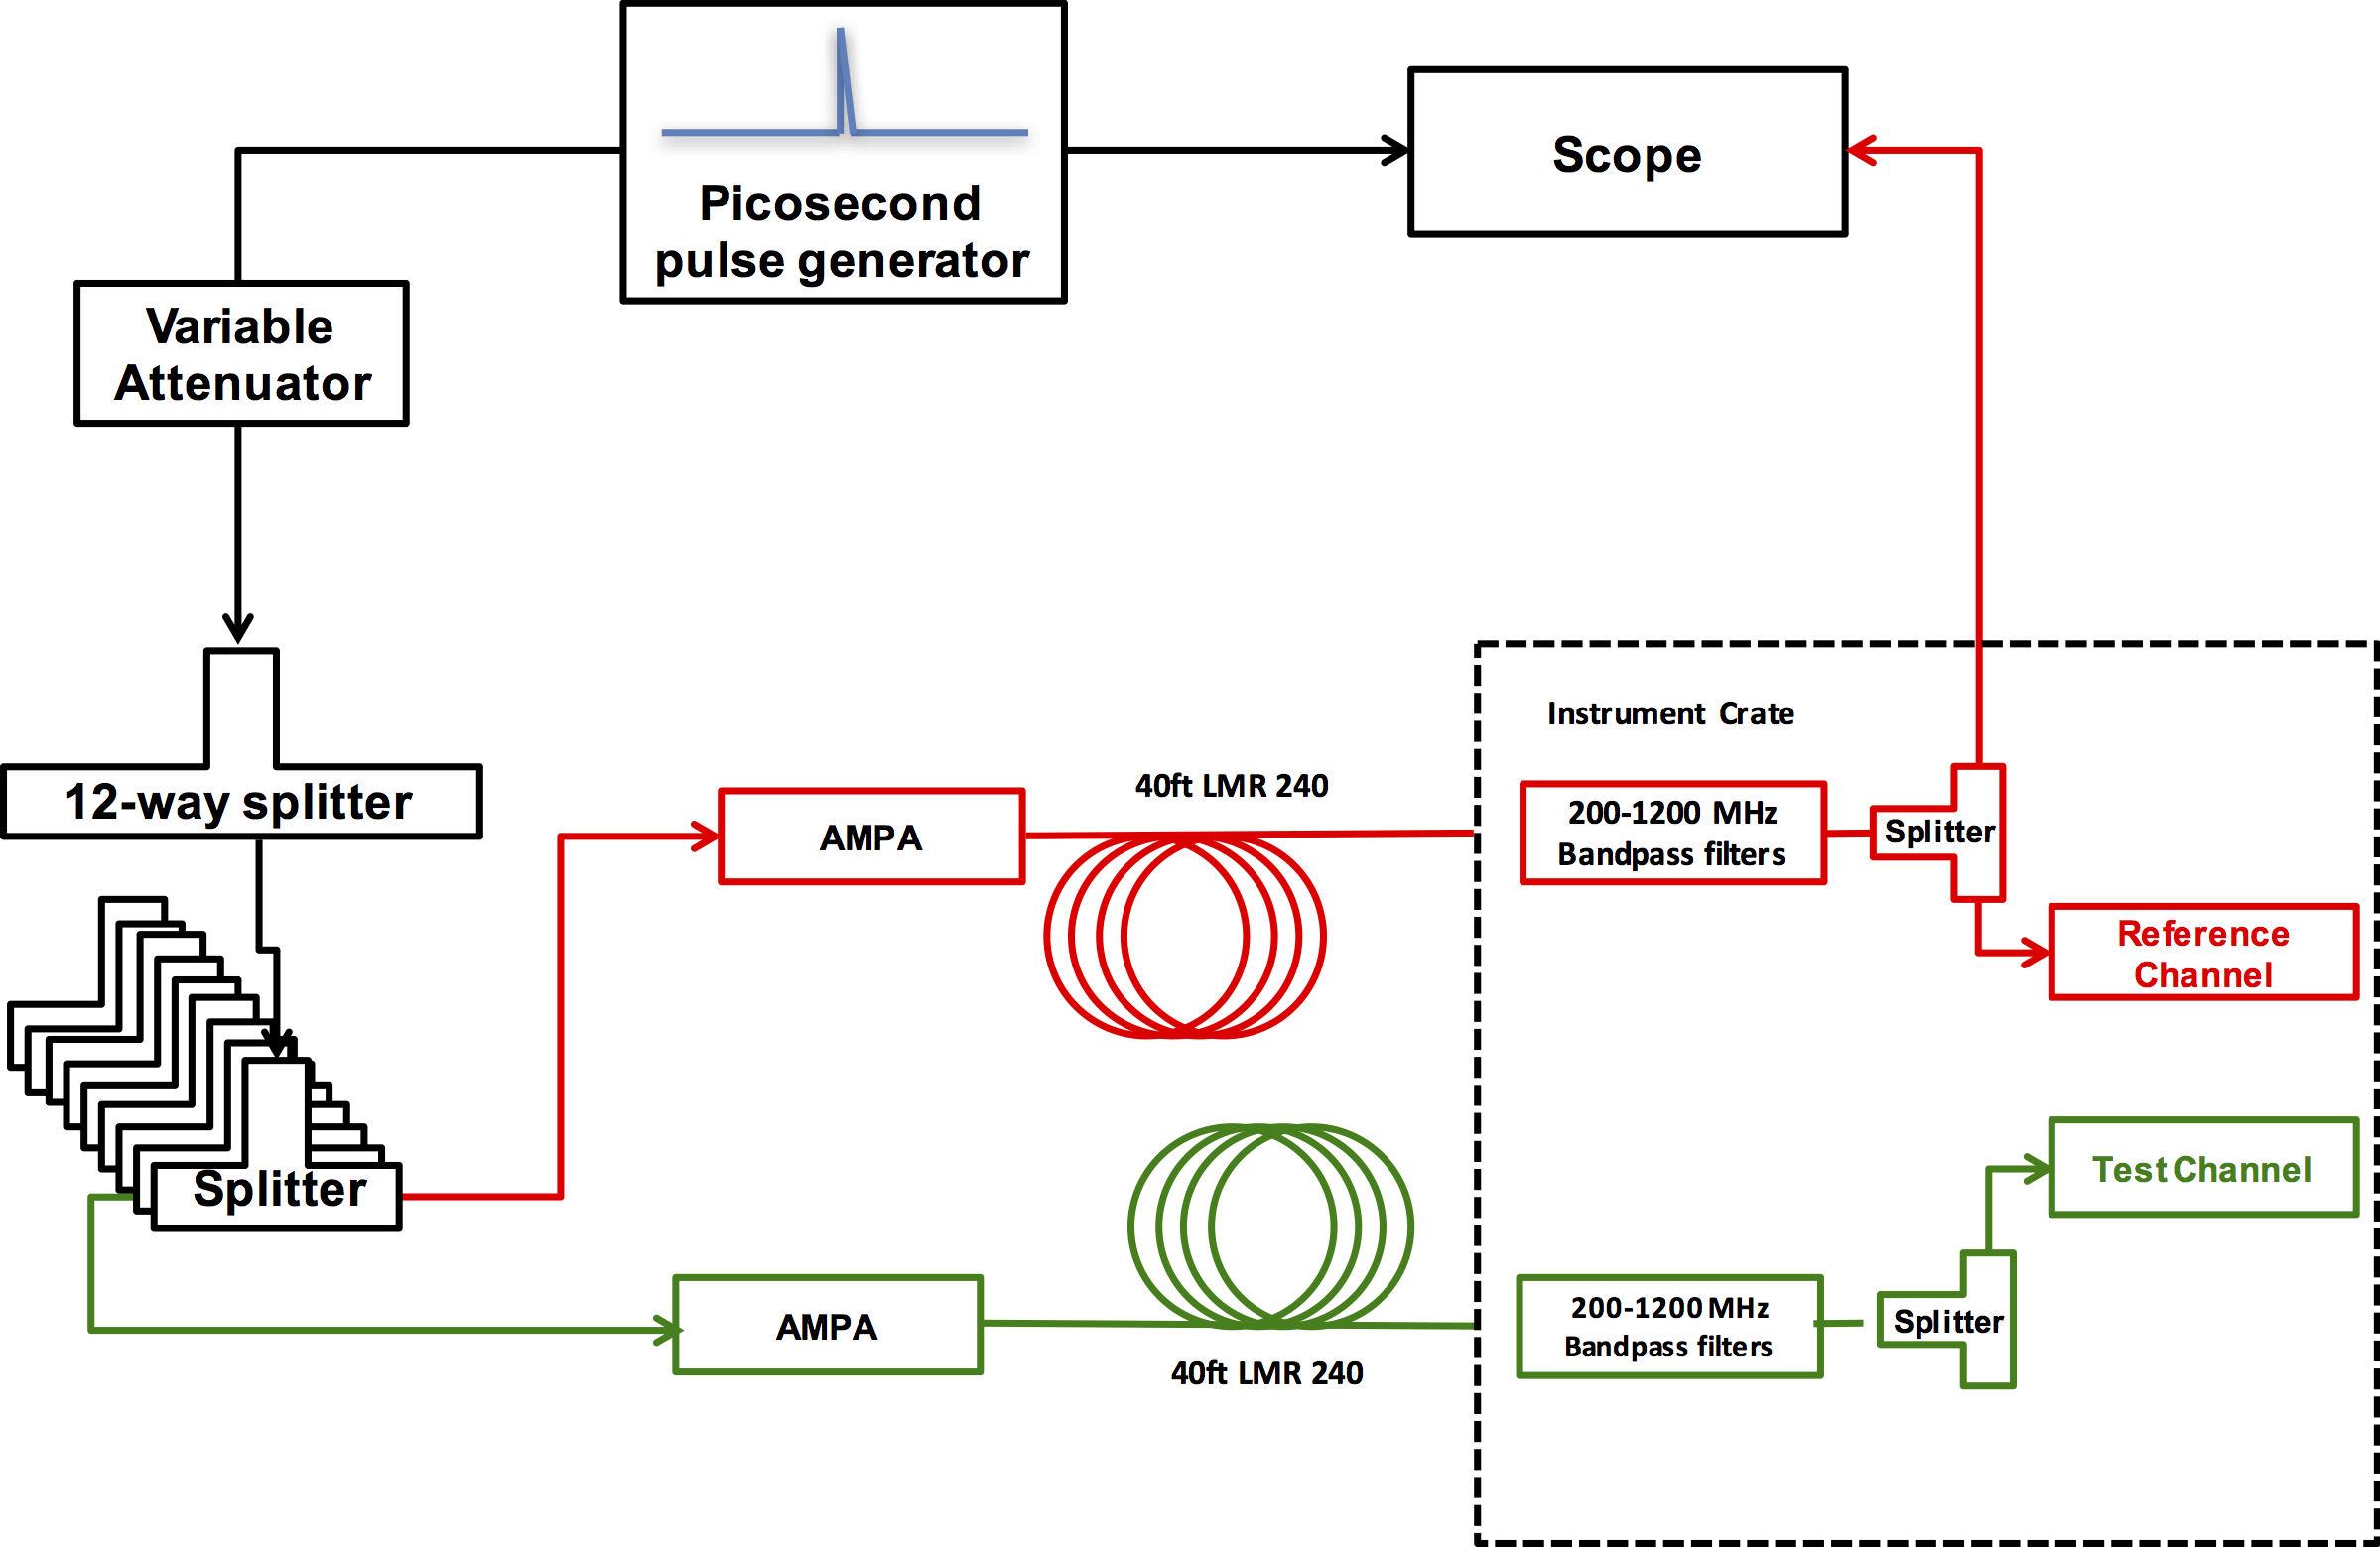
\includegraphics[width=.8\linewidth]{./Figs/TriggerEfficiencyScanSetup.png}
  \caption{Trigger efficiency scans setup in Antarctica before the ANITA-III flight. The signals from the trigger are sent to the oscilloscope via the red line and recorded.}
  \label{fig:scan_setup}
\end{figure}

To simulate the trigger efficiency scan setup, the signals
measured at the oscilloscope (see Figure~\ref{fig:scan_setup}) 
are inserted (with appropriate attenuation) into the same six channels as used
in the hardware efficiency scans.
These go through the trigger/digitizer path and produce ANITA
data-like outputs.
%When simulating trigger efficiency scans, constant power
%thresholds corresponding to 450\,kHz scalers are used for all channels.

The signals are recorded at the trigger and the digitizer paths
are used to validate the simulation.
Figure~\ref{fig:scan_snr} shows a comparison of the measured SNR in
data and simulation at the trigger (left) and at
the digitizer (right) as a function of the variable attenuation used
during the scan.
The SNR is calculated as the ratio of half of the peak-to-peak of the
time domain signal to the RMS of the last part of the waveform.
The measured SNR in the digitizer path generally has higher errors compared to the SNR in the trigger path, because the ANITA digitizer has on average a
2.6\,GHz sampling rate, whereas the trigger path is measured with a
fast oscilloscope. 

\begin{figure}[!h]\centering
  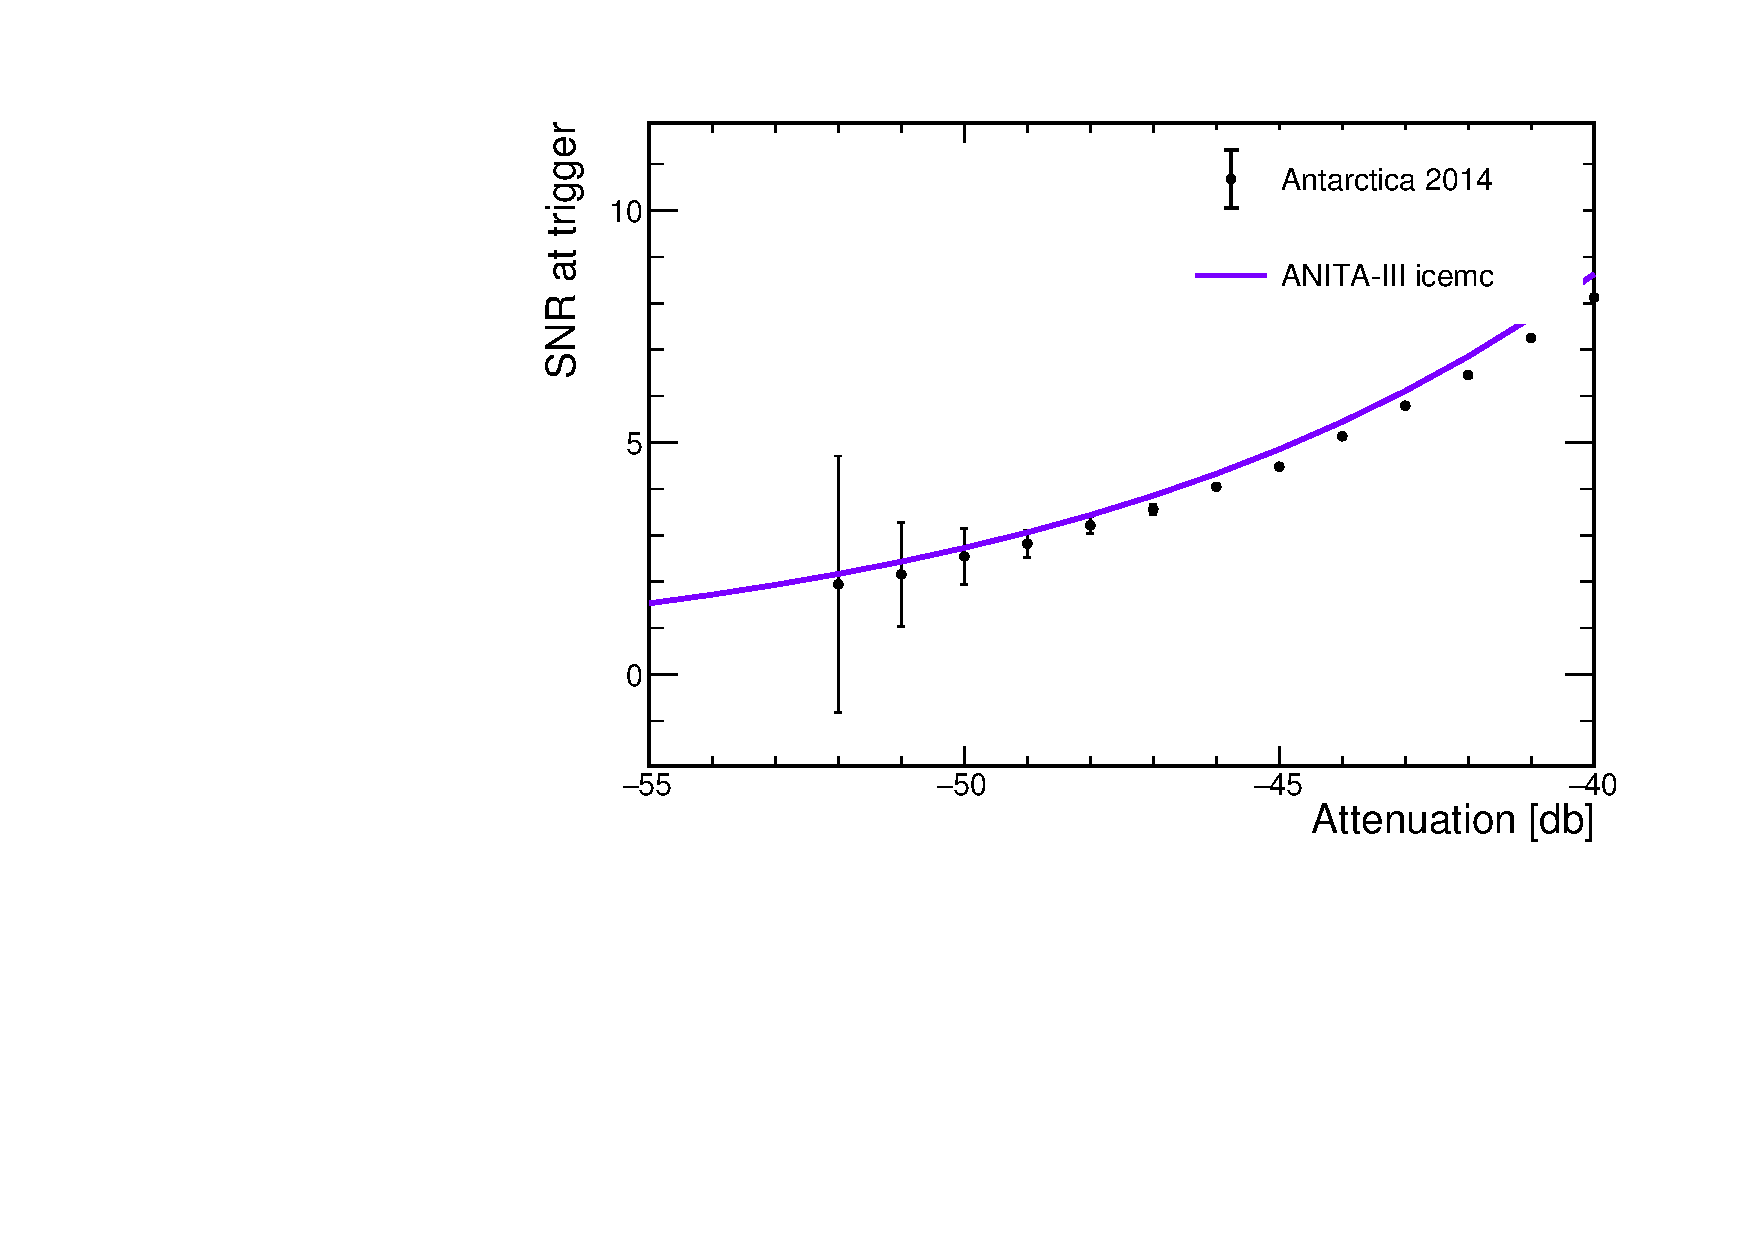
\includegraphics[width=.45\linewidth]{./Figs/EfficiencyScanNoDelaysA3_snrTriggerVSattenuation.pdf} 
  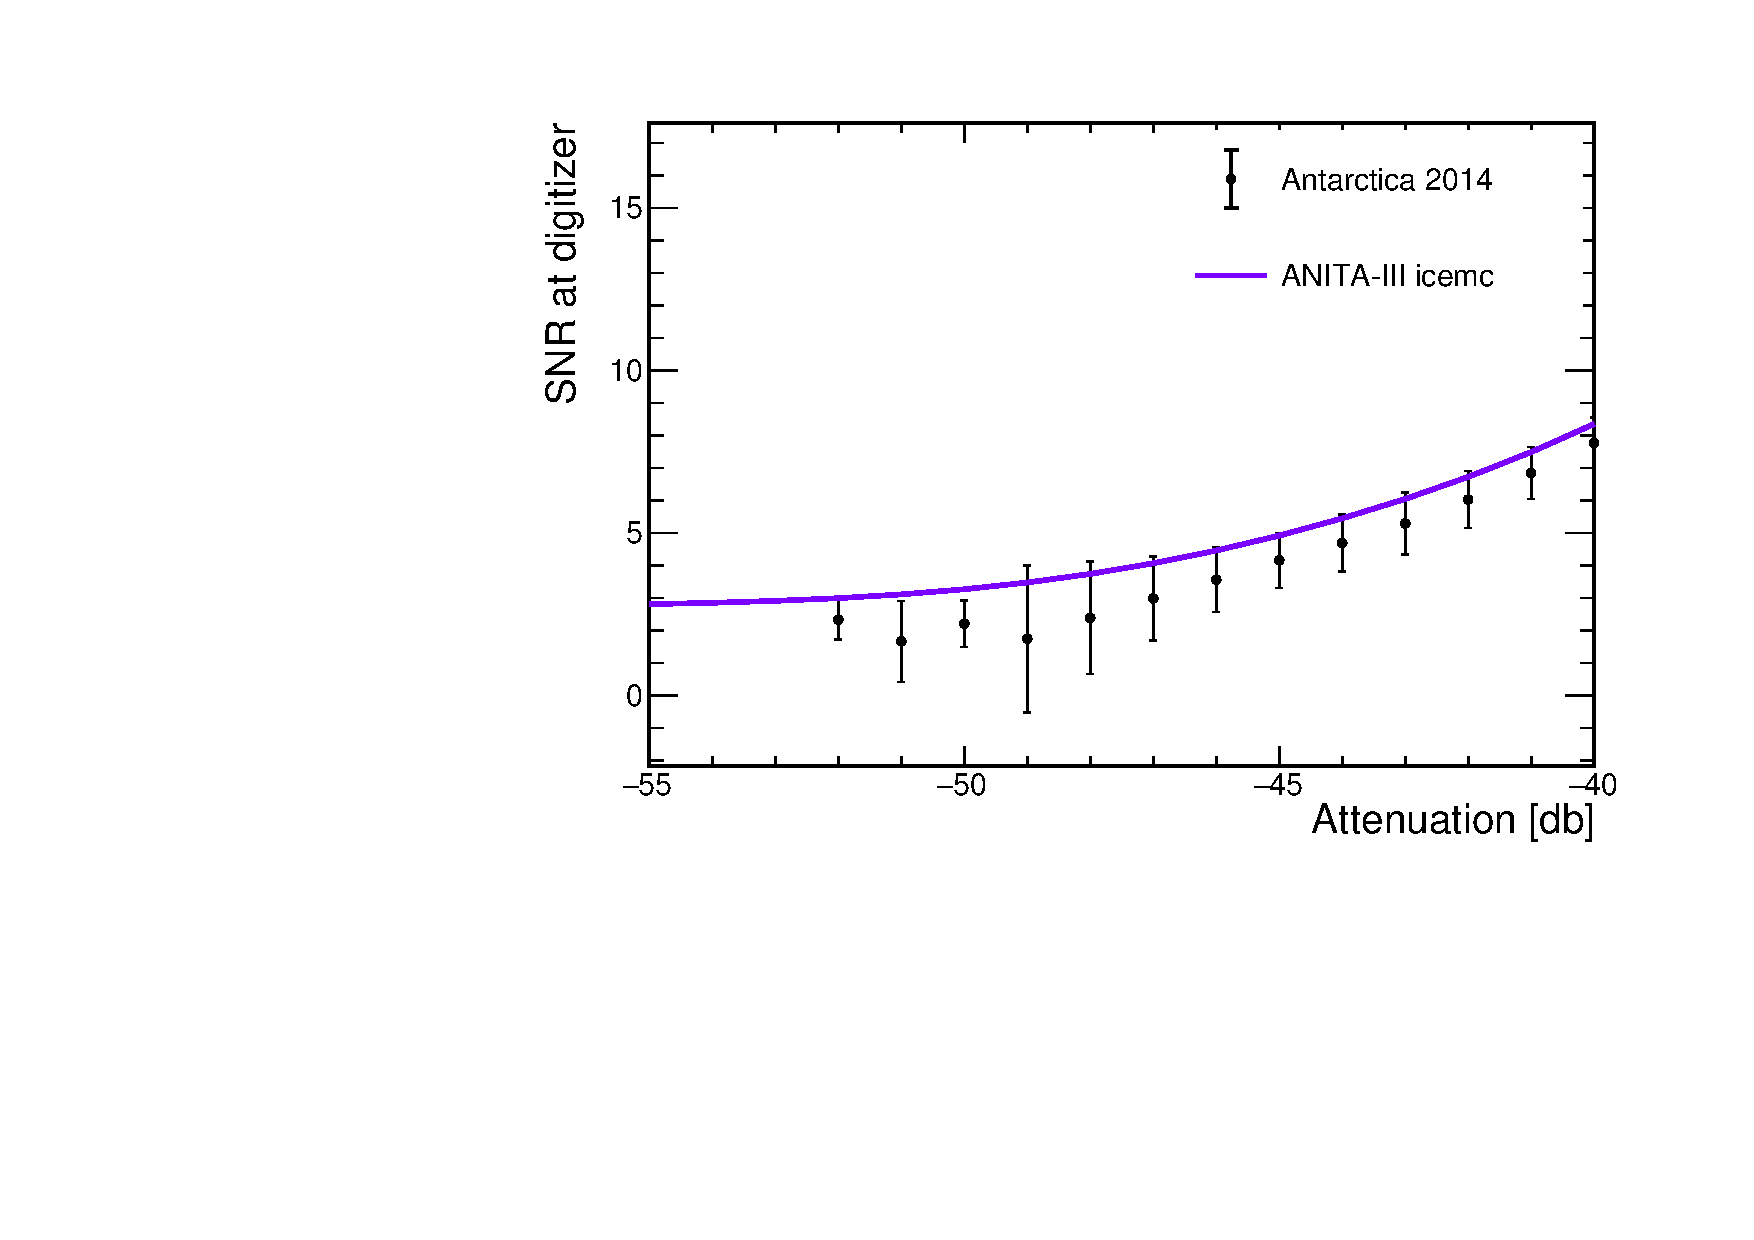
\includegraphics[width=.45\linewidth]{./Figs/EfficiencyScanNoDelaysA3_snrDigitizerVSattenuation.pdf}
  \caption{SNR measured at the trigger (left) and digitizer (right) as
  a function of the variable attenuation applied during the trigger
  efficiency scans. The data points were measured in 2014 in Antarctica prior to the
  ANITA-III flight.
}
  \label{fig:scan_snr}
\end{figure}

Figure~\ref{fig:scans}~(left) shows a comparison between data and simulation of a trigger efficiency scan for the ANITA-III payload.
The trigger efficiency is plotted as a function of the SNR
measured in the trigger path.

Before the ANITA-IV flight, a similar set of measurements was collected.
A data and simulation comparison of the trigger efficiency for the ANITA-IV instrument is shown in Figure~\ref{fig:scans}~(right).

\begin{figure}[!h]\centering
  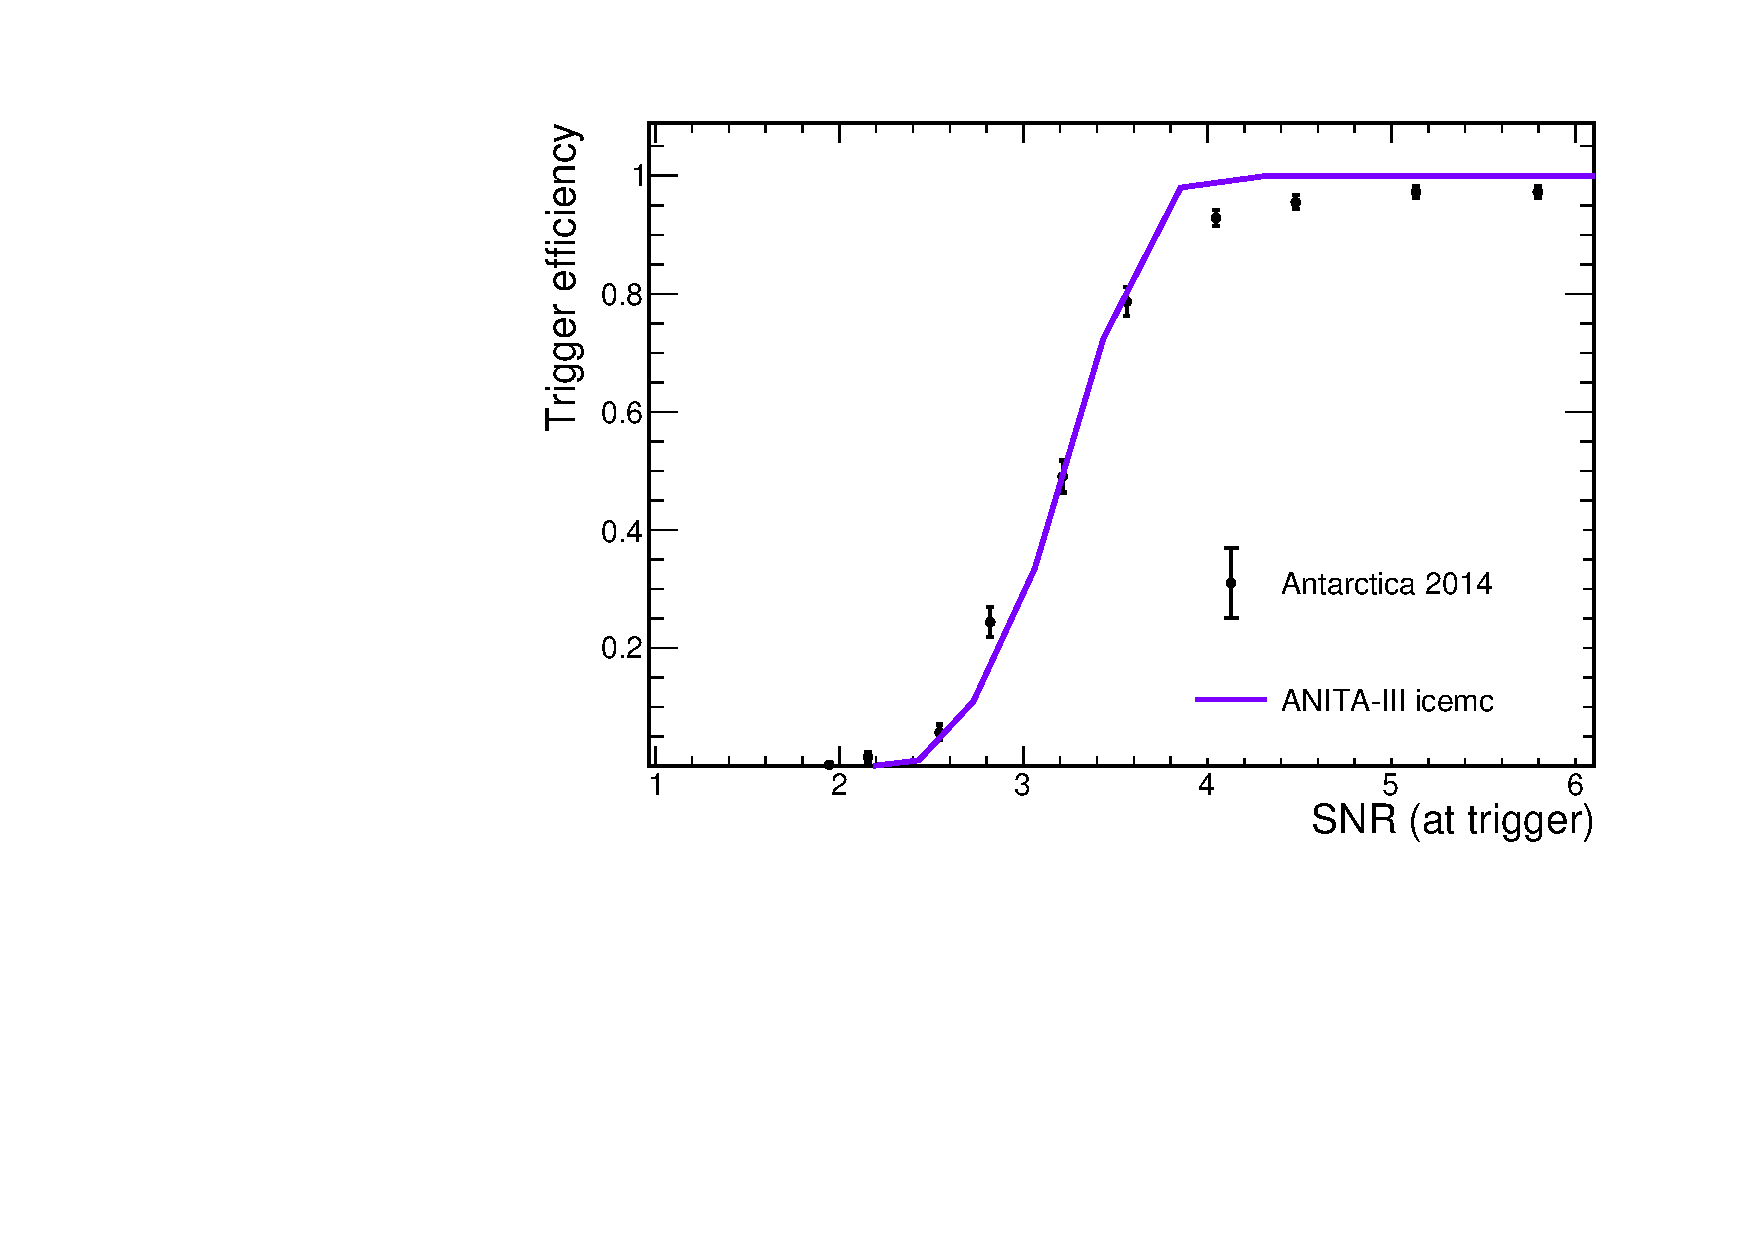
\includegraphics[width=.45\linewidth]{./Figs/EfficiencyScanNoDelaysA3_efficiencyVSsnrTrigger.pdf}
    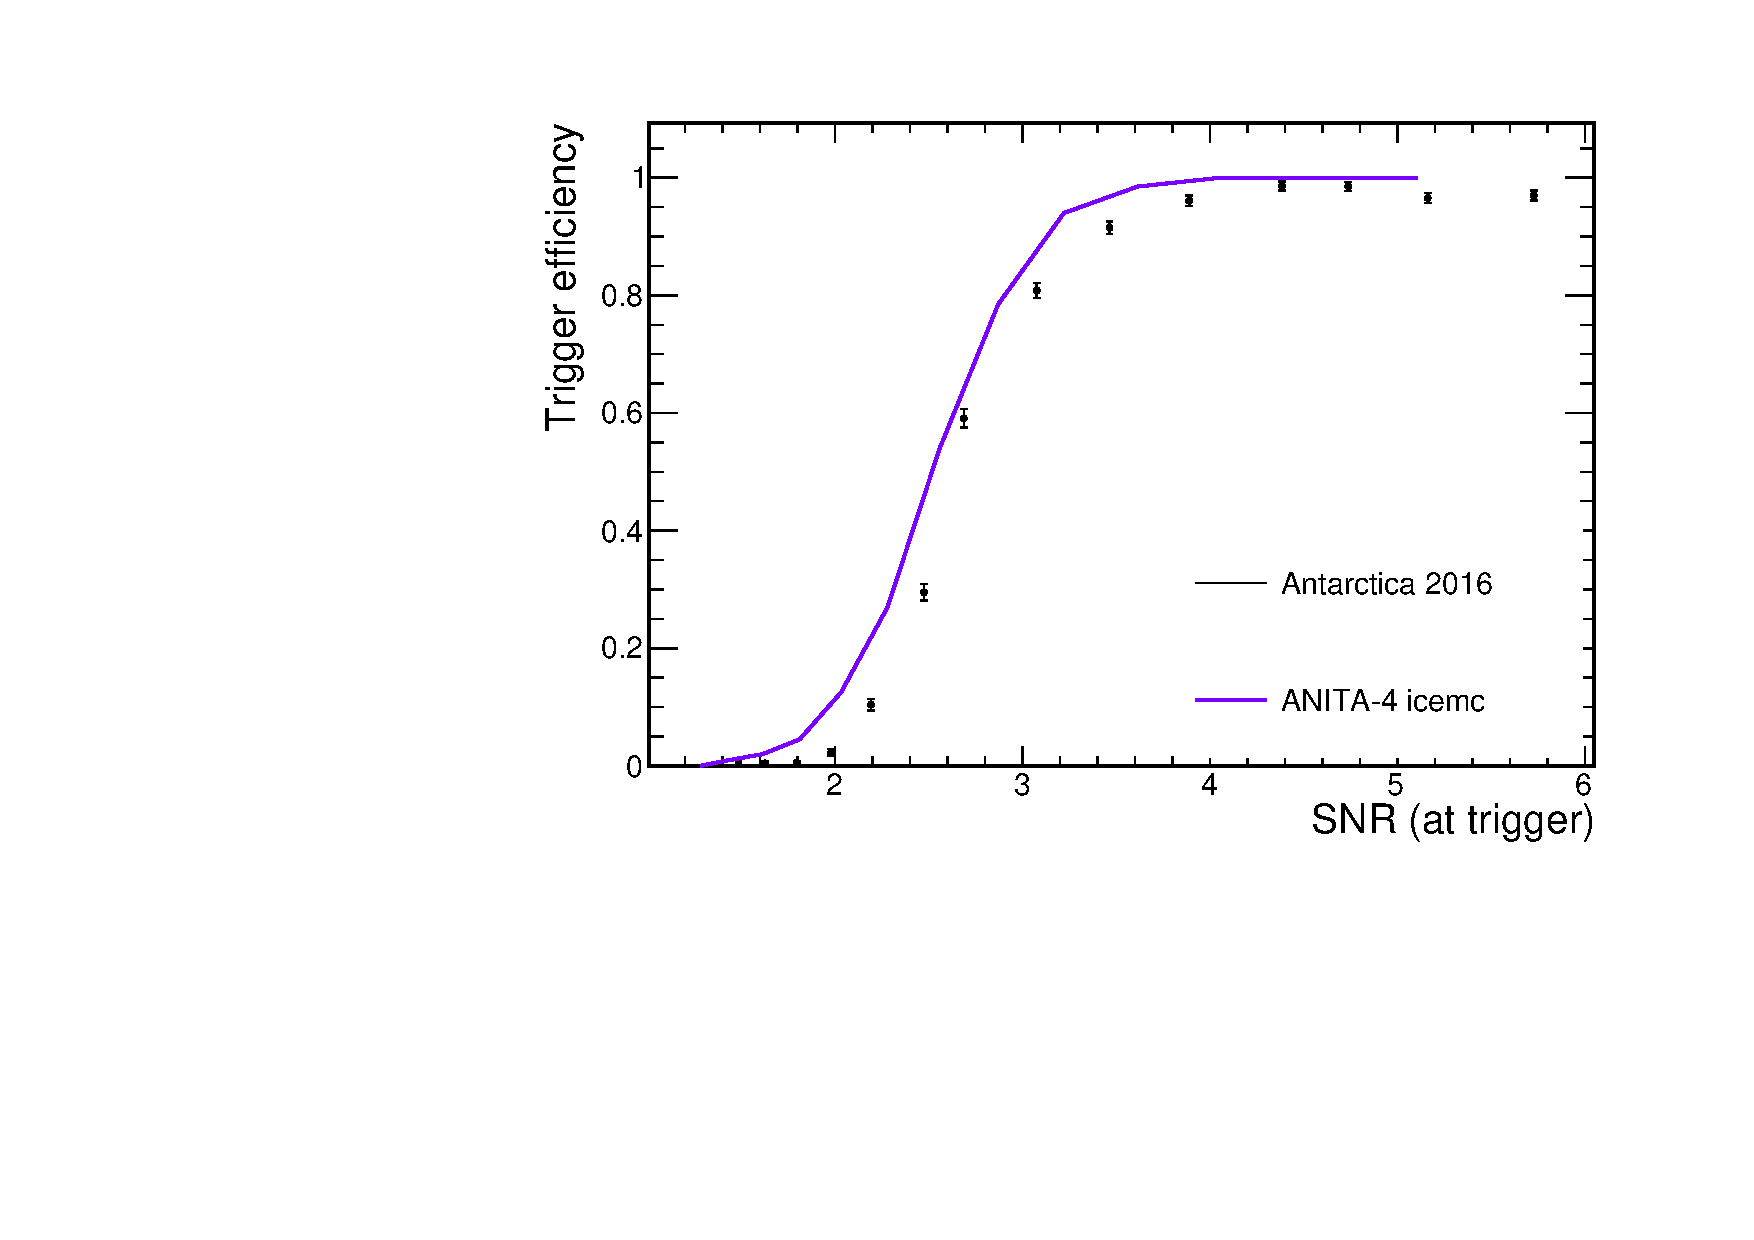
\includegraphics[width=.45\linewidth]{./Figs/EfficiencyScanNoDelaysA4_efficiencyVSsnrTrigger.pdf}
  \caption{Comparison between data and simulation of a trigger efficiency scan for the ANITA-III (left) and ANITA-IV (right) instruments. 
    The trigger efficiency is plotted a function of the SNR
    measured at the oscilloscope for the data, and the SNR estimated in the trigger path for the simulation. 
    }
  \label{fig:scans}
\end{figure}


\subsection{Comparisons with flight measurements}
\label{subsec:validation_flight}
Data taken during the ANITA-III and ANITA-IV flights are used to validate 
the thermal noise, the trigger efficiency to a ground pulser, and the pointing reconstruction.

\subsubsection{Thermal noise validation}
\label{subsec:ANITA_validation_thermalNoise}
The simulation of thermal noise is validated using distributions of
the RMS of the simulated waveforms compared to a relatively quiet time
during the flights.
Figure~\ref{fig:RMSwaveform} shows the voltage RMS of noise-only waveforms produced
in \icemc compared with the ones coming from a quiet time during
the ANITA-III (left) and ANITA-IV (right) flights.

As the ANITA-III data contained a significant amount of carrier wave
contamination, a fair comparison of the data and simulation thermal noise is done after applying two notch filters to both datasets, improving the data and simulation agreement.
The remaining differences are due to continuous wave noise in the data that
could not be simply removed with two notch filters.

The ANITA-IV payload was less affected by carrier wave noise, as the TUFF boards were directly filtering out noisy frequencies, and the requirement of the coincidence between LCP and RCP signals to form a trigger ensured that only linearly polarized signals triggered the payload.
A direct comparison between the measured and simulated noise is seen in Figure~\ref{fig:RMSwaveform}~(right). 

\begin{figure}[!h]\centering
  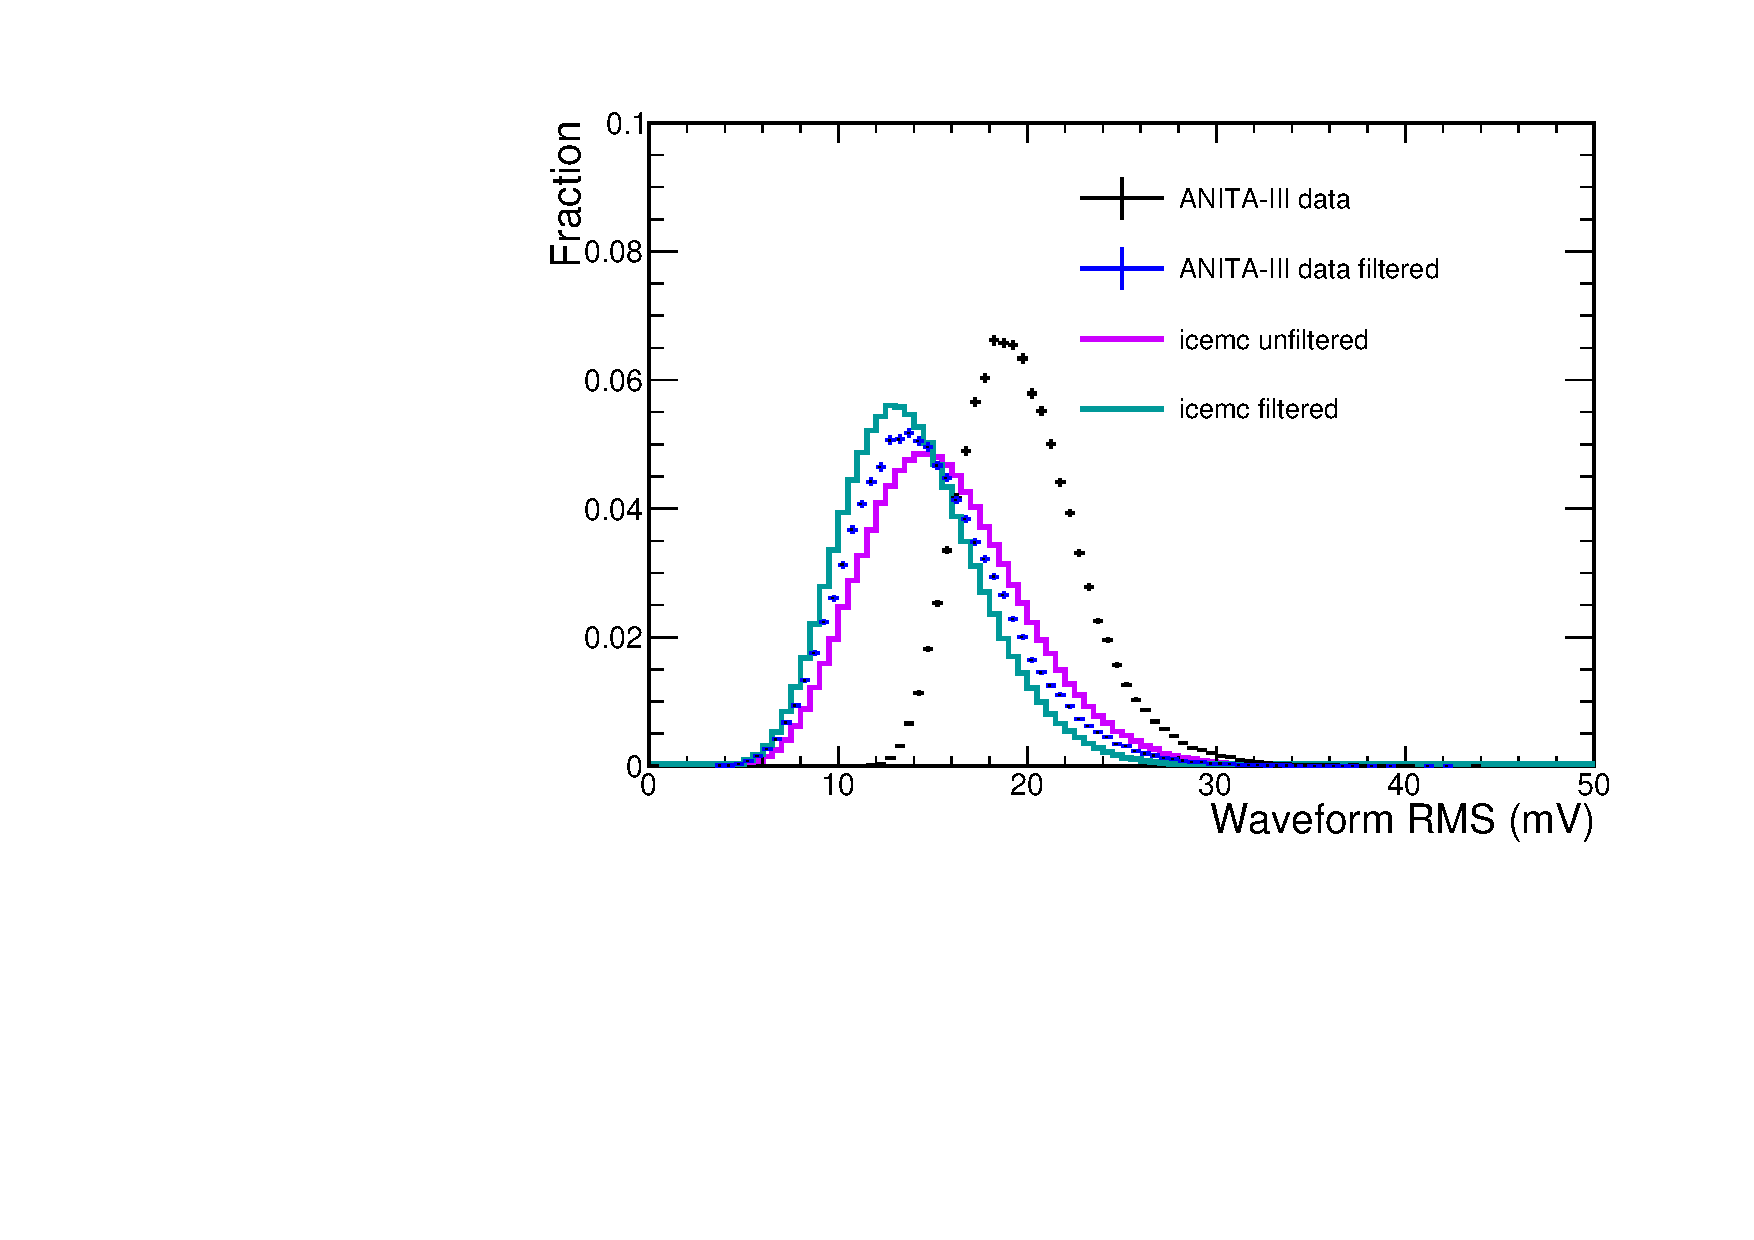
\includegraphics[width=.45\linewidth]{./Figs/ValidationThermalNoiseA3_RMSwaveform.pdf}
  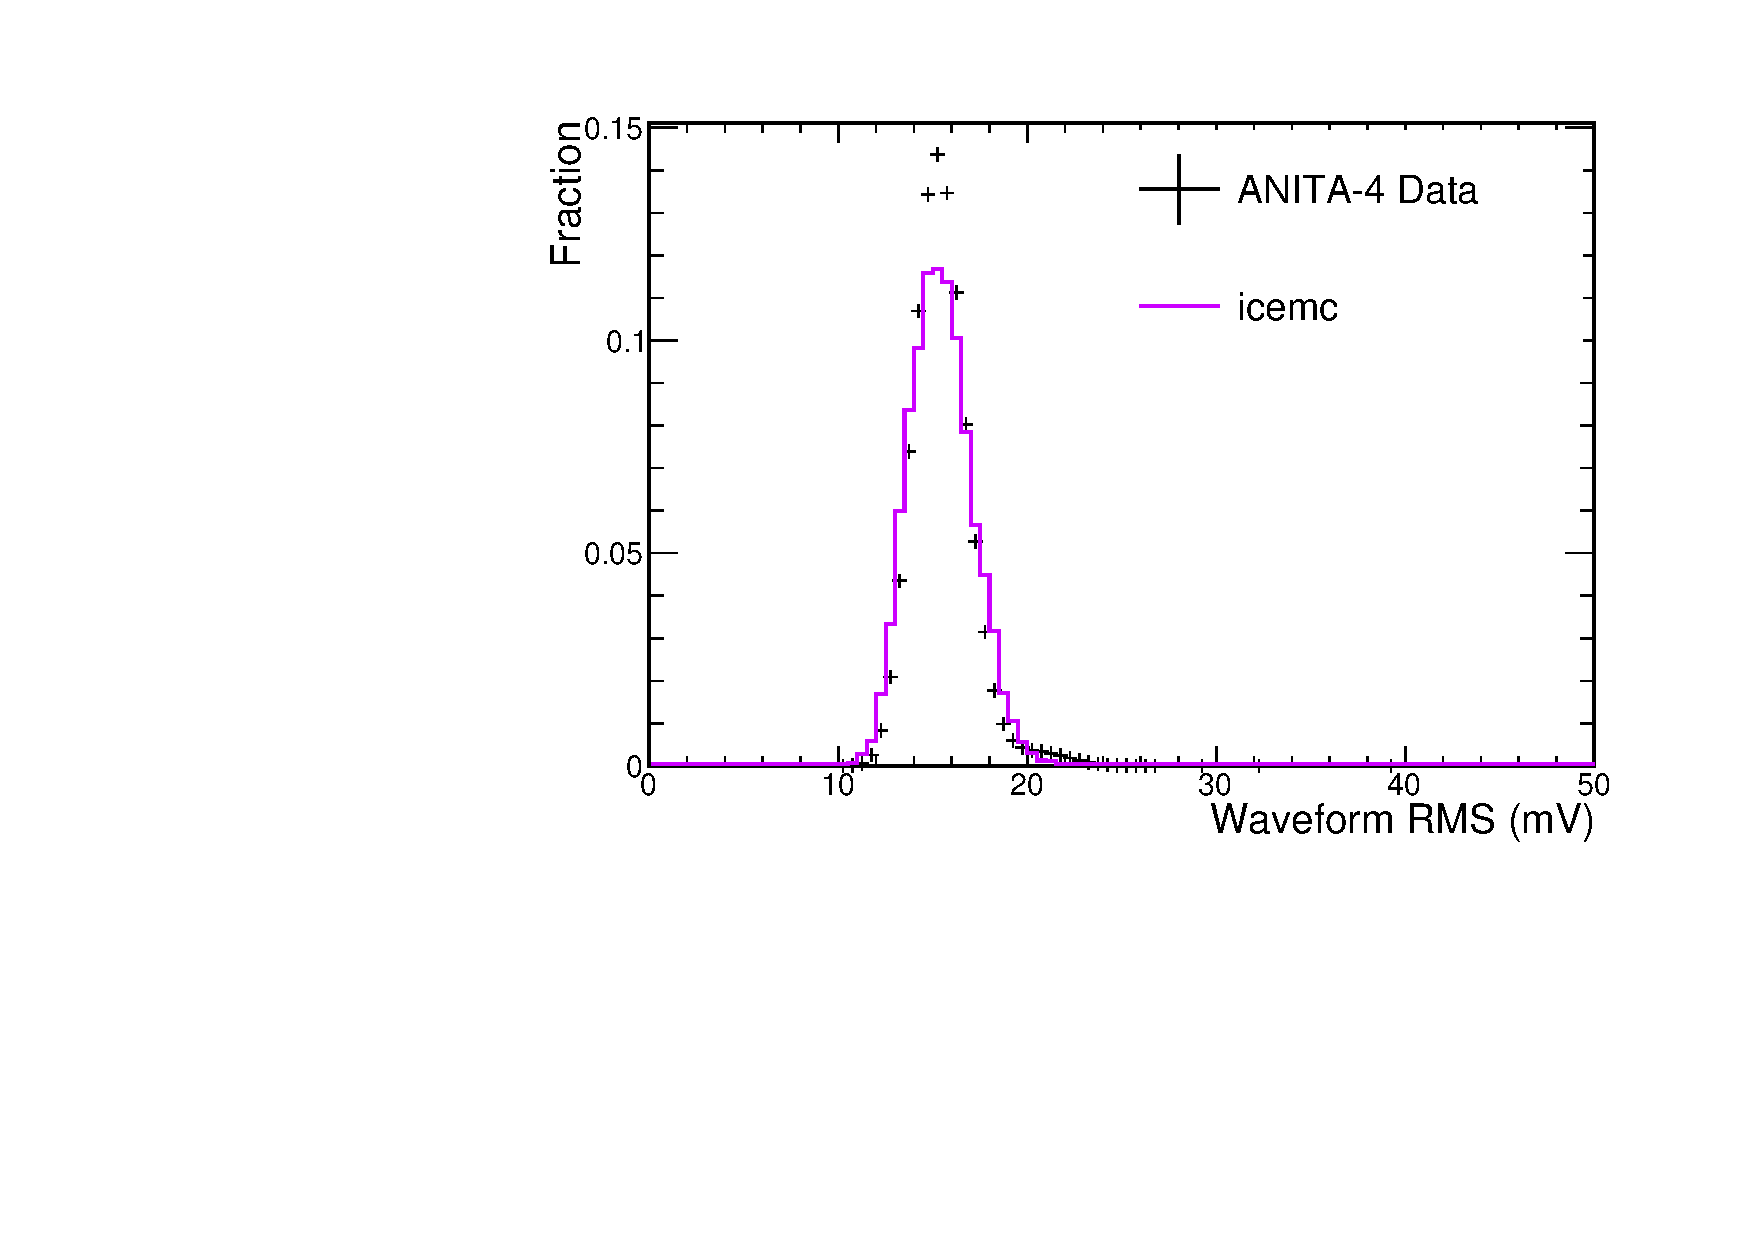
\includegraphics[width=.45\linewidth]{./Figs/ValidationThermalNoiseA4_RMSwaveform.pdf}

\caption{Thermal noise validation. Comparison of RMS of waveforms for an \icemc simulation and a relatively quiet period of the ANITA-III (left) and ANITA-IV (right) flights.
    The ANITA-III flight was affected by strong CW noise that for a better comparison has been filtered out.
    These distributions are normalized to equal area to better compare their shape.
  }
  \label{fig:RMSwaveform}
\end{figure}

As a second consistency check, the ANITA-III simulated thermal
noise is also used to produce Rayleigh fits (as described in
Subsection~\ref{subsec:ANITA_thermalNoise}) and shows complete overlap with the fits to the
ANITA-III quiet time.


\subsubsection{WAIS pulser model}
\label{subsec:wais}

As an additional validation, we model the calibration pulser that was located at the West Antarctic Ice Sheet (WAIS) field camp during the ANITA-III and ANITA-IV flights. The WAIS pulser consisted of a 6-kV FID brand pulser that generates a broadband impulse and drives a horizontally polarized antenna. The pulser was triggered on the GPS second with a known delay, permitting a measurement of the  ANITA trigger efficiency while the payload is in view of the pulser.

The antenna used at WAIS is a custom design based on a quad-slot model, for which the slots of the antenna are parallel to the ground. The antenna was installed $\sim$1~m below the surface of the snow. Similar to a discone, the bottom portion of the antenna acts as a reflector, and the angles of the taper on both the reflector and the upper cone tunes the orientation of the peak gain. This design is a scaled down version of the VHF antenna used as a low frequency extension to ANITA-III. 

The WAIS antenna response was modelled using NEC antenna modeling software~\cite{nec}. Figure~\ref{fig:waisPulser} shows the peak gain for each frequency, the associated phase at that frequency, and the reflection coefficient, $\Gamma(f)$, from this antenna model. We then model the electric field (Figure~\ref{fig:waisPulser}d) generated by the WAIS pulser by convolving the NEC model of the antenna with measurements of the voltage generated by the FID pulser on an oscilloscope. The electric field at 1\,m from the pulser, $E(f)$, results from relating the power density radiated by the antenna to the power density generated by the pulser with a characteristic impedance $Z_{c}$ and voltage $V(f)$ at the pulser, accounting for loss from imperfect antenna matching between the antenna and the pulser, the magnitude and phase of the gain, $G(f)$, propagation loss, and the impedance of free space, $Z_0$:

\begin{equation}
|E(f)| = \sqrt{\frac{|V(f)|^2}{8 Z_c} (1 -|\Gamma(f)|^2 ) \frac{Z_0}{2\pi (1~\textrm{m})^2} G}
\end{equation}

The simulation treats the electric field shown in Figure~\ref{fig:waisPulser} as originating from a source at the location of the WAIS pulser. Figure~\ref{fig:waisEff} shows the efficiency of the ANITA-III payload to generate a trigger from pulses coming from WAIS divide. The simulation efficiency does not asymptote to 1 at high SNR, as it also includes inefficiencies due to the channel masking and the instrument dead time. 

\begin{figure}
\centering
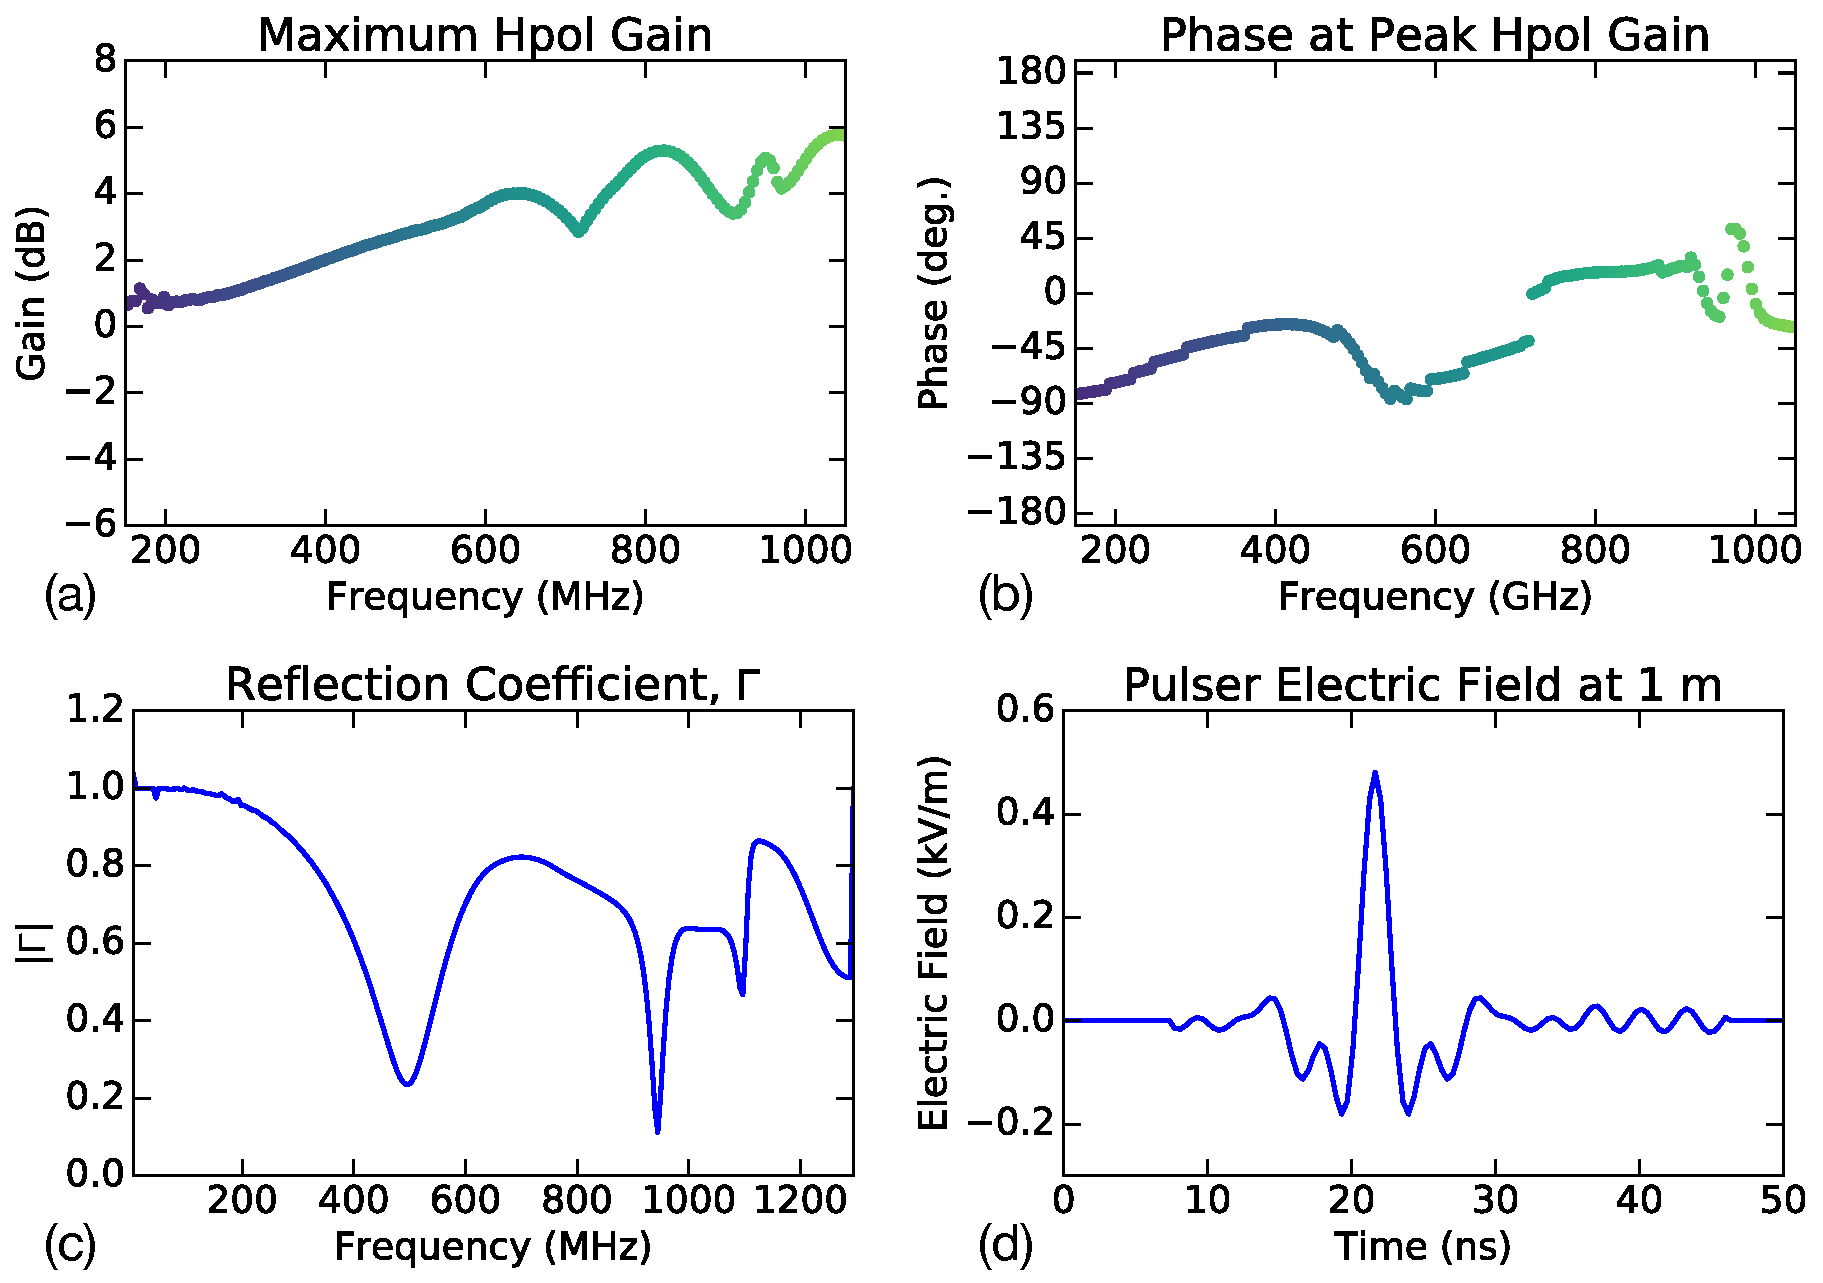
\includegraphics[width=\linewidth]{./Figs/waisPulser.pdf}
\caption{Characterization of the ANITA-III horizontally polarized antenna used in the WAIS pulser.}
\label{fig:waisPulser}
\end{figure}

\begin{figure}
\centering
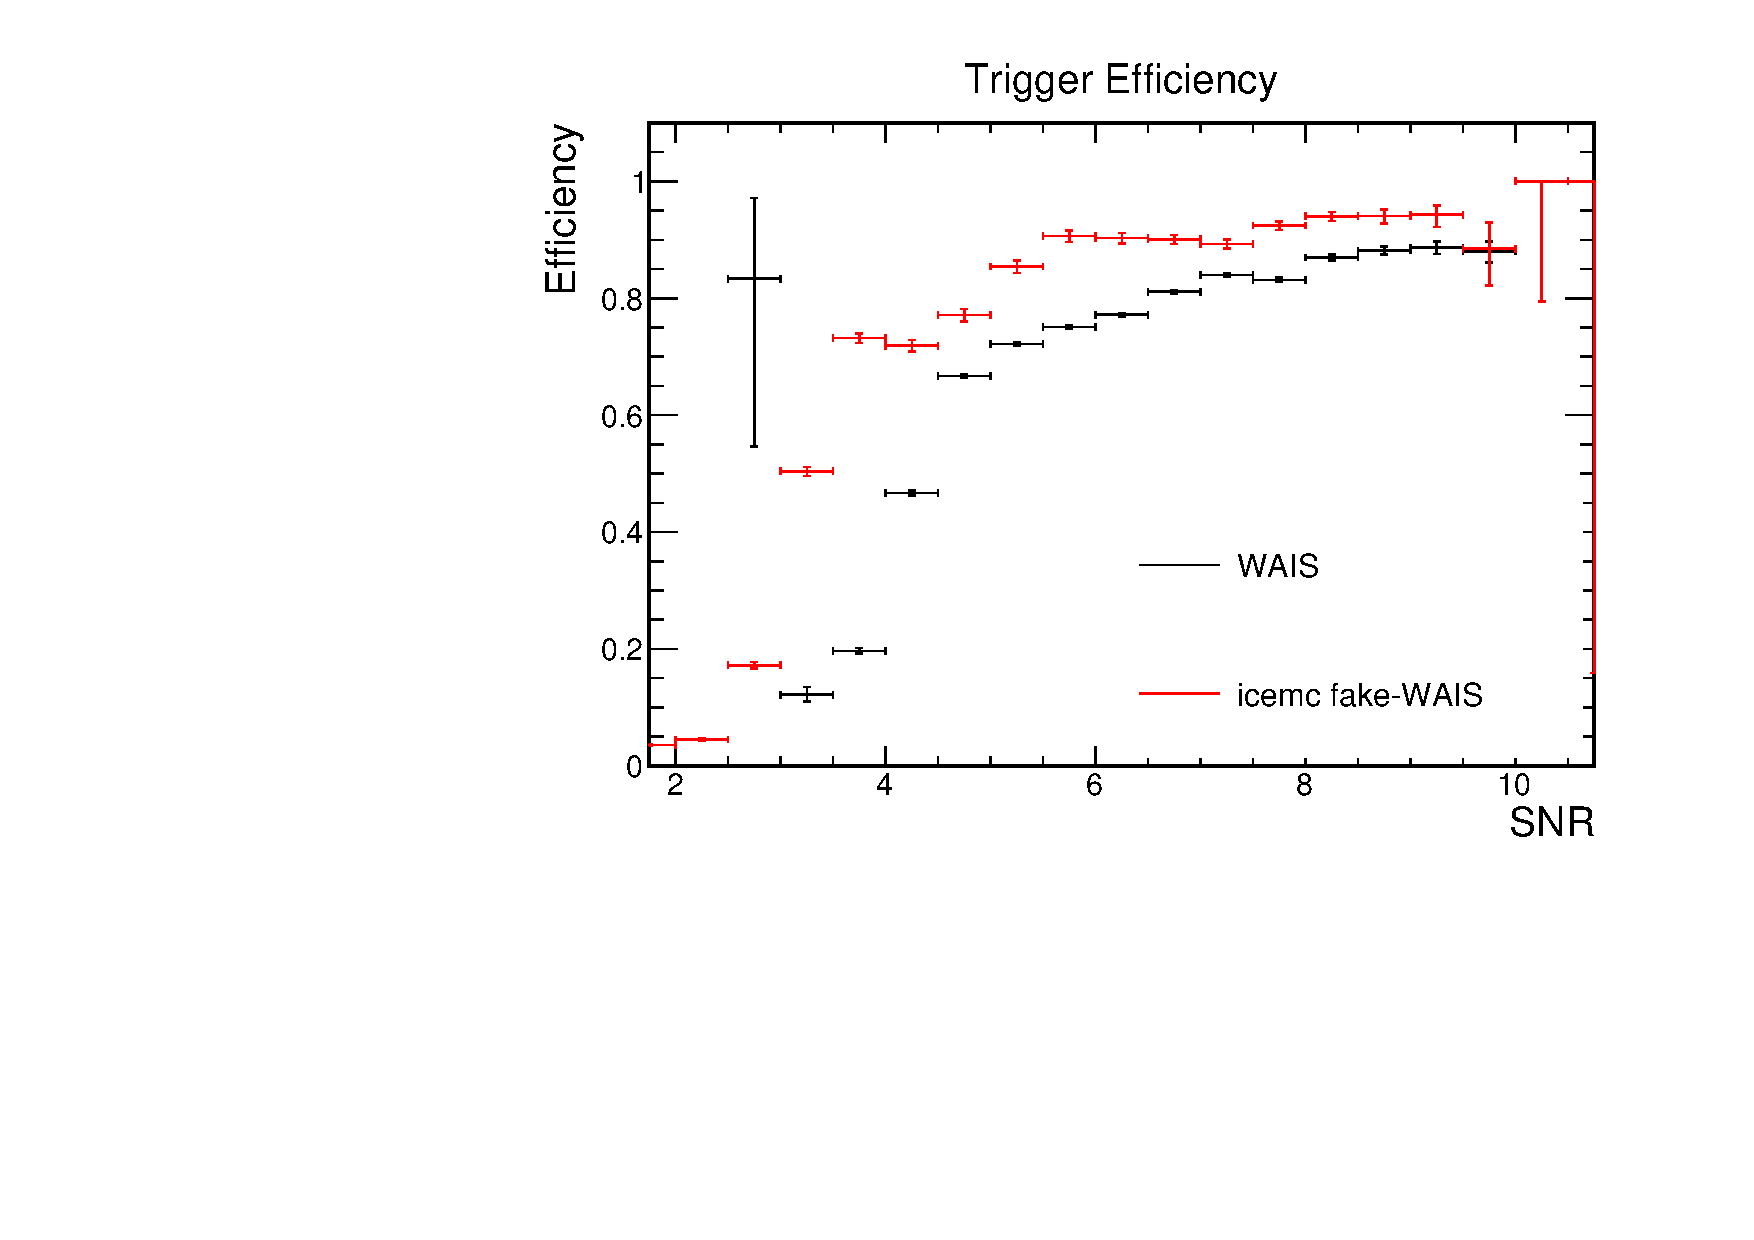
\includegraphics[width=.5\linewidth]{./Figs/Efficiency_WAIS.pdf}
\caption{ANITA-III trigger efficiency to a pulser coming from the WAIS divide station as a function of SNR.}
\label{fig:waisEff}
\end{figure}

\subsubsection{Reconstruction validation}
\label{subsec:ANITA_validation_reconstruction}
To fully validate the simulation, a large sample of simulated
neutrinos is produced following the cosmogenic neutrino flux arising from a mixed cosmic-ray composition as modeled by Kotera et al.~\cite{kotera}.
Simulated waveforms from different triggering channels are
cross-correlated to form a pointing map in the ANITA payload
coordinates, azimuth ($\phi_{\mathrm{meas}}$) and elevation
($\theta_{\mathrm{meas}}$). 
The peak of the correlation map is then compared to the expected
azimuth ($\phi_{\mathrm{theory}}$) and elevation
($\theta_{\mathrm{theory}}$), calculated from the true neutrino interaction point.
Details of our reconstruction and analysis can be found in our
previous publications~\cite{ANITA1paper,ANITA2paper,romero2015interferometric}.

